\documentclass[letterpaper,12pt]{article}
\usepackage{tabularx} % extra features for tabular environment
\usepackage{amsmath}  % improve math presentation
\usepackage{graphicx} % takes care of graphic including machinery
\usepackage[margin=1in,letterpaper]{geometry} % decreases margins
\usepackage{cite} % takes care of citations
\usepackage{longtable}
\usepackage{booktabs}
\usepackage[final]{hyperref} % adds hyper links inside the generated pdf file
\hypersetup{
	colorlinks=true,       % false: boxed links; true: colored links
	linkcolor=blue,        % color of internal links
	citecolor=blue,        % color of links to bibliography
	filecolor=magenta,     % color of file links
	urlcolor=blue         
}
\usepackage{blindtext}
\usepackage{caption}
\captionsetup[table]{skip=10pt}
%++++++++++++++++++++++++++++++++++++++++


\begin{document}

\title{Classify Images Using Deep Learning}
\author{Michele Antonazzi}
\date{\today}
\maketitle

\begin{abstract}
In this work, we perform a multi-classification task over images using deep learning models. The aim is to evaluate the neural networks' performances in relation with their type, architecture and hyper-parameters. The models tested are FFNN (feed-forward neural network) and CNN (convolutional neural network). 
\end{abstract}

\section{Introduction}
In the real world, there are a lot of different tasks that are too
complicated to be modeled by a conventional algorithm. Some problems
indeed may have a wide amount of data difficult to analyze. In this
case, build a specific algorithm means to understand the complex
patterns and the hidden correlations between the data. Instead, other
tasks may be influenced by a lot of external factors that generate a
large quantity of similar but different data. These factors are not easy
to model, especially considered all together, and often they are not a
priori known. This means that an algorithm performs well only in a
controlled environment, that respects specific preconditions. On the
other hand, if it is applied in the real world, the algorithm may
encounter data that it cannot correctly analyze. A particular field of
Computer Science is particularly suitable to solve these situations:
machine learning (ML). It represents a family of algorithms that learn
automatically through experience. These algorithms are not designed for
a specific task but they are general purposes so they can be used to
solve each type of task. The principle behind machine learning is the
following: each real phenomenon can be modeled as an unknown
mathematical function which can be approximate by a machine learning
algorithm. In particular, they build a mathematical model based on
sample data, known as training data, to make decisions or predictions
without being explicitly programmed to do so. This means that the data
play a central role in machine learning: they must be able to correctly
define the model behind the task. First of all, they must be sufficient
in number to generalize the problem, especially if the data have high
dimensionality. Secondly, they must be well-formed, in terms of the
range of values, scale, and distribution. Often a preprocessing
procedure is necessary to modify the data before being used by a
learning machine to improve its performance. There are three main
approaches to machine learning, depending on the nature and the type of
data available to a learning machine. The first is called
\emph{supervised learning} and consists in presenting to the learning
model the inputs with the correct outputs. The goal is to learn a
general function that maps inputs to outputs. Another machine learning
technique is \emph{unsupervised learning} where the input is not
associated with labels, leaving to the learning machine the task of
finding the data structure. Discovering the hidden patterns of data can
be a goal itself or the purpose can be the generation of new data with
similar characteristics. The last category is called \emph{reinforcement
learning} and occurs when a computer program interacts with a real
environment in which it must perform a certain task. The leaning machine
is provided by feedback which is analogous to rewards and it tries to
maximize them, as it navigates the specific problem space. Machine
learning algorithms are often used in computer vision tasks, like object
classification, object detection, motion analysis, and many others. In
the last few years, the state of the art methods to perform object
classification use machine learning, in particular \emph{deep learning.}
Deep learning is based on artificial neural networks, inspired by the
biological neural network that composed the animal brains. Specifically
to computer vision, the convolutional neural networks (CNNs) are
particularly suitable for analyzing images. They are able to learn how
to extract the features using the convolutional layers and,
subsequently, use these features in a space invariant way to better
generalize the data. In this work, it is performed a
multi-classification task over images. This task is performed using deep
learning models. The aim is to study the neural network performances
based on their type, their architecture, and their hyper-parameters. In
particular, the model tested is the feed-forward neural network (FFNN)
and the convolutional neural network (CNN).
\newpage
\section{Experimental setup}\label{header-n31}

The aim of this project is to evaluate the performances of deep networks
in an image multi-classification task. More in detail, it consists into
map fruit and vegetable images over ten classes: \emph{apple},
\emph{banana}, \emph{plum}, \emph{pepper}, \emph{cherry}, \emph{grape},
\emph{tomato}, \emph{potato}, \emph{pear}, and \emph{peach}.

\subsection{Dataset}\label{header-n33}

The dataset consists of a wide series of images that depict different
types of fruit and vegetables. It is downloadable by following this
\href{https://www.kaggle.com/moltean/fruits}{link}. The original dataset
is already divided into training and test set. For each set, each type
of fruit and vegetable is divided according to its main characteristics.
For instance, the fruit type "apple" can be divided into a lot of
sub-categories according to its variety (apple Golden, apple Granny
Smith, apple Pink Lady, etc) and its color (yellow, red, green, etc). In
the dataset, for each type-feature pair, there is a folder that contains
the related pictures. The dataset is not used as is but it is modified
and reorganize to perform the assigned task. First of all, the split
between training and test set is removed in order to compose a single
set of images. Secondly, the sub-types of fruit and vegetables are
grouped together. This means that all apple sub-types belonging to the
same class. Finally, only the 10 requested types of fruit and vegetables
are considered(apple, banana, plum, pepper, cherry, grape, tomato,
potato, pear, and peach), the others are removed. Now the dataset is
composed of ten folders that contain the images relating to the ten
classes. The figure below shows the ten classes.

\begin{figure}[h!]
\centering
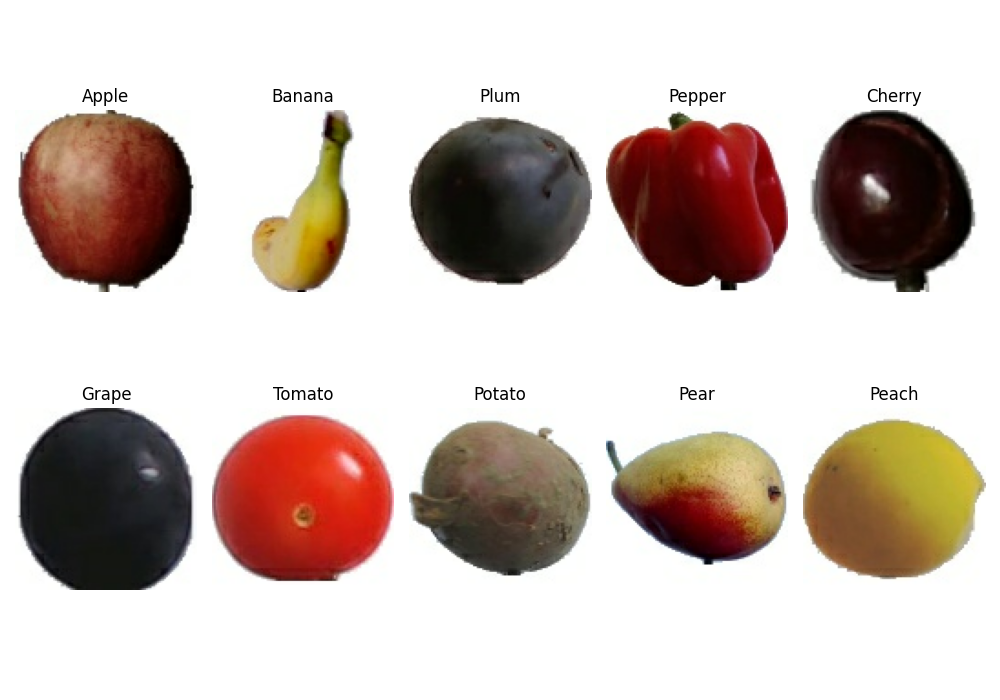
\includegraphics[width=0.9\linewidth]{../images/fruit-categories.png}
\caption{The classes of picture which the models have to predict}
\end{figure}

To better understand how the dataset is composed, the following table
and graphic show the number of samples for each class and the total
amount of pictures

\begin{longtable}[]{@{}ll@{}}
\toprule
\textbf{Class} & \textbf{N. of samples}\tabularnewline
\midrule
\endhead
Apple & 8538\tabularnewline
Banana & 1258\tabularnewline
Cherry & 4592\tabularnewline
Grape & 4565\tabularnewline
Peach & 1640\tabularnewline
Pear & 6070\tabularnewline
Pepper & 3304\tabularnewline
Plum & 1766\tabularnewline
Potato & 2404\tabularnewline
Peach & 6810\tabularnewline
\textbf{Total} & \textbf{40947}\tabularnewline
\bottomrule
\caption{The amount of samples for each class}
\end{longtable}

\begin{figure}[h!]
\centering
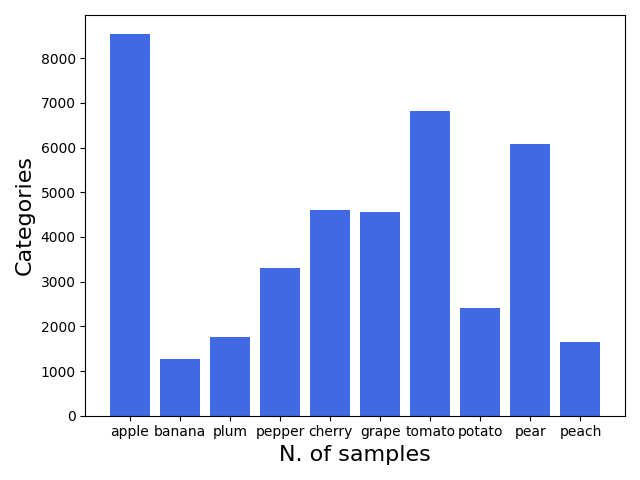
\includegraphics[width=0.9\linewidth]{../images/n_samples.png}
\caption{The amount of samples for each class}
\end{figure}

\subsection{Data preprocessing}\label{header-n75}

The problem data (the images) have to be properly elaborated before
being used by models. The data preprocessing phase aims to make the
dataset easier to analyze, to increase the models' performance, and
reduce the training time. The preprocessing pipeline, applied for each
dataset picture, is composed of two steps:

\begin{itemize}
\item
  \textbf{scaling:} the image is resized form 100x100 pixels to 32x32
  pixels using the bilinear interpolation algorithm
\item
  \textbf{normalization:} the pixels RGB channel values, originally in
  the {[}0, 255{]} range, are standardized to be in the {[}0, 1{]}
  range.
\end{itemize}

\subsection{Experiments evaluation}\label{header-n82}

After the preprocessing pipeline, the data are ready to pass to the
learning models. Cross-validation is used to evaluate the models'
performances, in particular the Hold-out technique. This method consists
into split the dataset in two separate sets: the training set (used to
train the leaning machines) and the test set (used to evaluate the
models' performance). In this case, the split is 80\% and 20\% for
training and test set. The union between them form an holdout. The
experiments are executed over 20 different holdouts. The
\href{https://scikit-learn.org/stable/modules/generated/sklearn.model_selection.StratifiedShuffleSplit.html}{method}
used to compute the holdouts is implemented in the sklearn library. This
method randomly separates the training and test set indices, preserving
the percentage of samples for each class. It is set with 42 as a random
state parameter. To numerically evaluate the models the following
metrics are used:

\begin{itemize}
\item
  \textbf{loss function value}: the value of the model's loss function
\item
  \textbf{accuracy:} the ration between the correct predictions and the
  total number of samples.
\end{itemize}

The final results are the mean and the standard deviation of the metrics
obtained by the learning machines using each holdouts (both for training
and validation phases). These results and the related conclusions are
finally validated using the Wilcoxon Signed-Rank test with a p-value
threshold of 0.01. It is a non-parametric statistical test to compare
hypotheses made on repeated measures. In addiction, for each model, the
trend of the metrics during the training phase are plotted to understand
how the model learns during the succession of epochs. The metrics are
calculated both on the training and test sets of the first holdout.
\newpage
\section{Models}\label{header-n90}

This section reports the architecture and hyper-parameters of the
neural networks used to classy the images. In particular, the model
tested are feed-forward neural networks (FFNNs) and convolutional neural
networks (CNNs).

\subsection{Feed-forward neural network}\label{header-n92}

The feed-forward neural network is the first and simplest type of
artificial neural network. The information moves in only one direction,
forward, from the input nodes, through the hidden nodes, and to the
output nodes. The layers of neurons are fully connected, in the sense
that each neuron of a layer is connected to all neurons of the previous
and next layers. The following tables specify the architecture and the
hyper-parameters for each model. In particular, for each layer, the
number of neurons (called \emph{Units}) and the activation function are
reported. Instead, for the hyper-parameters, the tables contain the
weight estimator and its learning rate, the loss function, the number of
epochs, and the batch size.

The first model (called \emph{Perceptron}) is a classical neural network
with the simplest architecture: the single layer perceptron. It consists
of a single layer which is also the output layer. Its purpose is to
examine the network performance with the given dataset to build better
models.

\begin{longtable}[]{@{}llll@{}}
	\toprule
	\textbf{Layers} & \textbf{Type} & \textbf{Units} & \textbf{Activation}\tabularnewline
	\midrule
	\endhead
	Layer 1 & Input & - & -\tabularnewline
	Layer 2 & Flatten & - & -\tabularnewline
	Layer 3 & Dense & 10 & Linear\tabularnewline
	\bottomrule
	\caption{\emph{Perceptron} architecture}
\end{longtable}

\begin{longtable}[]{@{}ll@{}}
	\toprule
	\textbf{Parameter} & \textbf{Value}\tabularnewline
	\midrule
	\endhead
	Weight estimator & adam\tabularnewline
	Learning rate & 0.001\tabularnewline
	Loss function & sparse categorical crossentropy\tabularnewline
	Epochs & 20\tabularnewline
	Batch size & 256\tabularnewline
	\bottomrule
	\caption{\emph{Perceptron} hyper-parameters}
\end{longtable}

\newpage

The second model is called \emph{FFNN}. It is similar to the first with
more complex architecture. In particular, this network has two hidden
layers.

\begin{longtable}[]{@{}llll@{}}
	\toprule
	\textbf{Layers} & \textbf{Type} & \textbf{Units} & \textbf{Activation}\tabularnewline
	\midrule
	\endhead
	Layer 1 & Input & - & -\tabularnewline
	Layer 2 & Flatten & - & -\tabularnewline
	Layer 3 & Dense & 64 & ReLU\tabularnewline
	Layer 4 & Dense & 32 & ReLU\tabularnewline
	Layer 5 & Dense & 10 & Linear\tabularnewline
	\bottomrule
	\caption{\emph{FFNN} architecture}
\end{longtable}

\begin{longtable}[]{@{}ll@{}}
	\toprule
	\textbf{Parameter} & \textbf{Value}\tabularnewline
	\midrule
	\endhead
	Weight estimator & adam\tabularnewline
	Learning rate & 0.001\tabularnewline
	Loss function & sparse categorical crossentropy\tabularnewline
	Epochs & 20\tabularnewline
	Batch size & 256\tabularnewline
	\bottomrule
	\caption{\emph{FFNN} hyper-parameters}
\end{longtable}

\subsection{Convolutional neural networks}\label{header-n186}

The next models are convolutional neural networks. This network at first
learns what are the data features using convolutional layers and
subsequently uses these features to label the data thanks to fully
connected layers. CNNs are often used to analyze visual images thanks to
their space invariant characteristics. The following tables specify the
architecture and the hyper-parameters for each model. In particular, for
each layer, the number of filters, the kernel size used by them, and the
activation function are reported. The kernel size is expressed with one
or two numbers based on the number of dimensions, while each number
indicates the length of its dimension. Instead, the hyper-parameters are
the same as those listed in the previous section.
\newpage
The first convolutional neural network is called \emph{CNN\_1}. Its
architecture is really simple, with a single convolutional layer (after
the input layer), a pooling layer (which implements the max operation),
and a dense layer (before the output layer).

\begin{longtable}[]{@{}lllll@{}}
	\toprule
	\textbf{Layers} & \textbf{Type} & \textbf{Filters} & \textbf{Kernel size} &
	\textbf{Activation}\tabularnewline
	\midrule
	\endhead
	Layer 1 & Input & - & - & -\tabularnewline
	Layer 2 & Conv2D & 2 & 3, 3 & ReLU\tabularnewline
	Layer 3 & MaxPooling2D & - & 2, 2 & -\tabularnewline
	Layer 4 & Flatten & - & - & -\tabularnewline
	Layer 5 & Dense & 64 & & ReLU\tabularnewline
	Layer 6 & Dense & 10 & & Linear\tabularnewline
	\bottomrule
		\caption{\emph{CNN\_1} architecture}
\end{longtable}

\begin{longtable}[]{@{}ll@{}}
	\toprule
	\textbf{Parameter} & \textbf{Value}\tabularnewline
	\midrule
	\endhead
	Weight estimator & adam\tabularnewline
	Learning rate & 0.001\tabularnewline
	Loss function & sparse categorical crossentropy\tabularnewline
	Epochs & 20\tabularnewline
	Batch size & 256\tabularnewline
	\bottomrule
	\caption{\emph{CNN\_1} hyper-parameters}
\end{longtable}

The second convolutional neural network (called \emph{CNN\_2}) is
similar to \emph{CNN\_1} but it has another pair of convolutional and
pooling layer.

\begin{longtable}[]{@{}lllll@{}}
	\toprule
	\textbf{Layers} & Type & \textbf{Filters} & \textbf{Kernel size} &
	\textbf{Activation}\tabularnewline
	\midrule
	\endhead
	Layer 1 & Input & - & - & -\tabularnewline
	Layer 2 & Conv2D & 4 & 3, 3 & ReLU\tabularnewline
	Layer 3 & MaxPooling2D & - & 2, 2 & -\tabularnewline
	Layer 4 & Conv2D & 2 & 3, 3 & ReLU\tabularnewline
	Layer 5 & MaxPooling2D & - & 2, 2 & -\tabularnewline
	Layer 6 & Flatten & - & - & -\tabularnewline
	Layer 7 & Dense & 64 & & ReLU\tabularnewline
	Layer 8 & Dense & 10 & & Linear\tabularnewline
	\bottomrule
		\caption{\emph{CNN\_2} architecture}
\end{longtable}

\newpage

\begin{longtable}[]{@{}ll@{}}
	\toprule
	\textbf{Parameter} & \textbf{Value}\tabularnewline
	\midrule
	\endhead
	Weight estimator & adam\tabularnewline
	Learning rate & 0.001\tabularnewline
	Loss function & sparse categorical crossentropy\tabularnewline
	Epochs & 20\tabularnewline
	Batch size & 256\tabularnewline
	\bottomrule
		\caption{\emph{CNN\_2} hyper-parameters}
\end{longtable}

The third model (called \emph{CNN\_3}) is more complex than the previous
one in its architecture. It has another pair of convolutional and
pooling layer.

\begin{longtable}[]{@{}lllll@{}}
	\toprule
	\textbf{Layers} & \textbf{Type} & \textbf{Filters} & \textbf{Kernel size} &
	\textbf{Activation}\tabularnewline
	\midrule
	\endhead
	Layer 1 & Input & - & - & -\tabularnewline
	Layer 2 & Conv2D & 8 & 3, 3 & ReLU\tabularnewline
	Layer 3 & MaxPooling & - & 2, 2 & -\tabularnewline
	Layer 4 & Conv2D & 4 & 3, 3 & ReLU\tabularnewline
	Layer 5 & MaxPooling2D & - & 2, 2 & -\tabularnewline
	Layer 6 & Conv2D & 2 & 3, 3 & ReLU\tabularnewline
	Layer 7 & MaxPooling2D & - & 2, 2 & -\tabularnewline
	Layer 8 & Flatten & - & - & -\tabularnewline
	Layer 9 & Dense & 64 & & ReLU\tabularnewline
	Layer 10 & Dense & 10 & & Linear\tabularnewline
	\bottomrule
		\caption{\emph{CNN\_3} architecture}
\end{longtable}

\begin{longtable}[]{@{}ll@{}}
	\toprule
	\textbf{Parameter} & \textbf{Value}\tabularnewline
	\midrule
	\endhead
	Weight estimator & adam\tabularnewline
	Learning rate & 0.001\tabularnewline
	Loss function & sparse categorical crossentropy\tabularnewline
	Epochs & 20\tabularnewline
	Batch size & 256\tabularnewline
	\bottomrule
		\caption{\emph{CNN\_3} hyper-parameters}
\end{longtable}

\newpage

The last convolutional neural networks is called \emph{CNN\_4}. It has
the same architecture that the \emph{CNN\_3} but its hyper-parameters
are different. In particular, the number of epochs rises to 50 and the
batch size goes down to 64.

\begin{longtable}[]{@{}lllll@{}}
	\toprule
	\textbf{Layers} & \textbf{Type} & \textbf{Filters} & \textbf{Kernel size} &
	\textbf{Activation}\tabularnewline
	\midrule
	\endhead
	Layer 1 & Input & - & - & -\tabularnewline
	Layer 2 & Conv2D & 8 & 3, 3 & ReLU\tabularnewline
	Layer 3 & MaxPooling & - & 2, 2 & -\tabularnewline
	Layer 4 & Conv2D & 4 & 3, 3 & ReLU\tabularnewline
	Layer 5 & MaxPooling2D & - & 2, 2 & -\tabularnewline
	Layer 6 & Conv2D & 2 & 3, 3 & ReLU\tabularnewline
	Layer 7 & MaxPooling2D & - & 2, 2 & -\tabularnewline
	Layer 8 & Flatten & - & - & -\tabularnewline
	Layer 9 & Dense & 64 & & ReLU\tabularnewline
	Layer 10 & Dense & 10 & & Linear\tabularnewline
	\bottomrule
		\caption{\emph{CNN\_4} architecture}
\end{longtable}

\begin{longtable}[]{@{}ll@{}}
	\toprule
	\textbf{Parameter} & \textbf{Value}\tabularnewline
	\midrule
	\endhead
	Weight estimator & adam\tabularnewline
	Learning rate & 0.001\tabularnewline
	Loss function & sparse categorical crossentropy\tabularnewline
	Epochs & 50\tabularnewline
	Batch size & 64\tabularnewline
	\bottomrule
		\caption{\emph{CNN\_4} hyper-parameters}
\end{longtable}

\section{Experimental results}\label{header-n500}

\subsection{Metrics over the holdouts}\label{header-n501}

In this section the experimental results are reported. For each metric
(loss function value and accuracy) there are a table and a plot to
confront the learning machine performance. Each metric is calculated for
each model for each holdout and the final results are the mean and the
standard deviation of the metrics obtained over the holdouts. The values
are reported for both training and testing phases.

\newpage
\textbf{Accuracy}

\begin{longtable}[]{@{}lll@{}}
\toprule
\textbf{Models} & \textbf{Training} & \textbf{Test}\tabularnewline
\midrule
\endhead
Perceptron & mean = 0.9665 & mean = 0.9633\tabularnewline
& STD = 0.0016 & STD = 0.0035\tabularnewline
FFNN & mean = 0.9993 & mean = 0.9987\tabularnewline
& STD = 0.0008 & STD = 0.0009\tabularnewline
CNN\_1 & mean = 0.9982 & mean = 0.9969\tabularnewline
& STD = 0.0012 & STD = 0.0022\tabularnewline
CNN\_2 & mean = 0.9854 & mean = 0.9839\tabularnewline
& STD = 0.0074 & STD = 0.007\tabularnewline
CNN\_3 & mean = 0.8814 & mean = 0.8797\tabularnewline
& STD = 0.0239 & STD = 0.0252\tabularnewline
CNN\_4 & mean = 0.9627 & mean = 0.961\tabularnewline
& STD = 0.031 & STD = 0.0314\tabularnewline
\bottomrule
\caption{Accuracy and its standard deviation results for training and test sets}
\end{longtable}

\begin{figure}[h!]
	\centering
	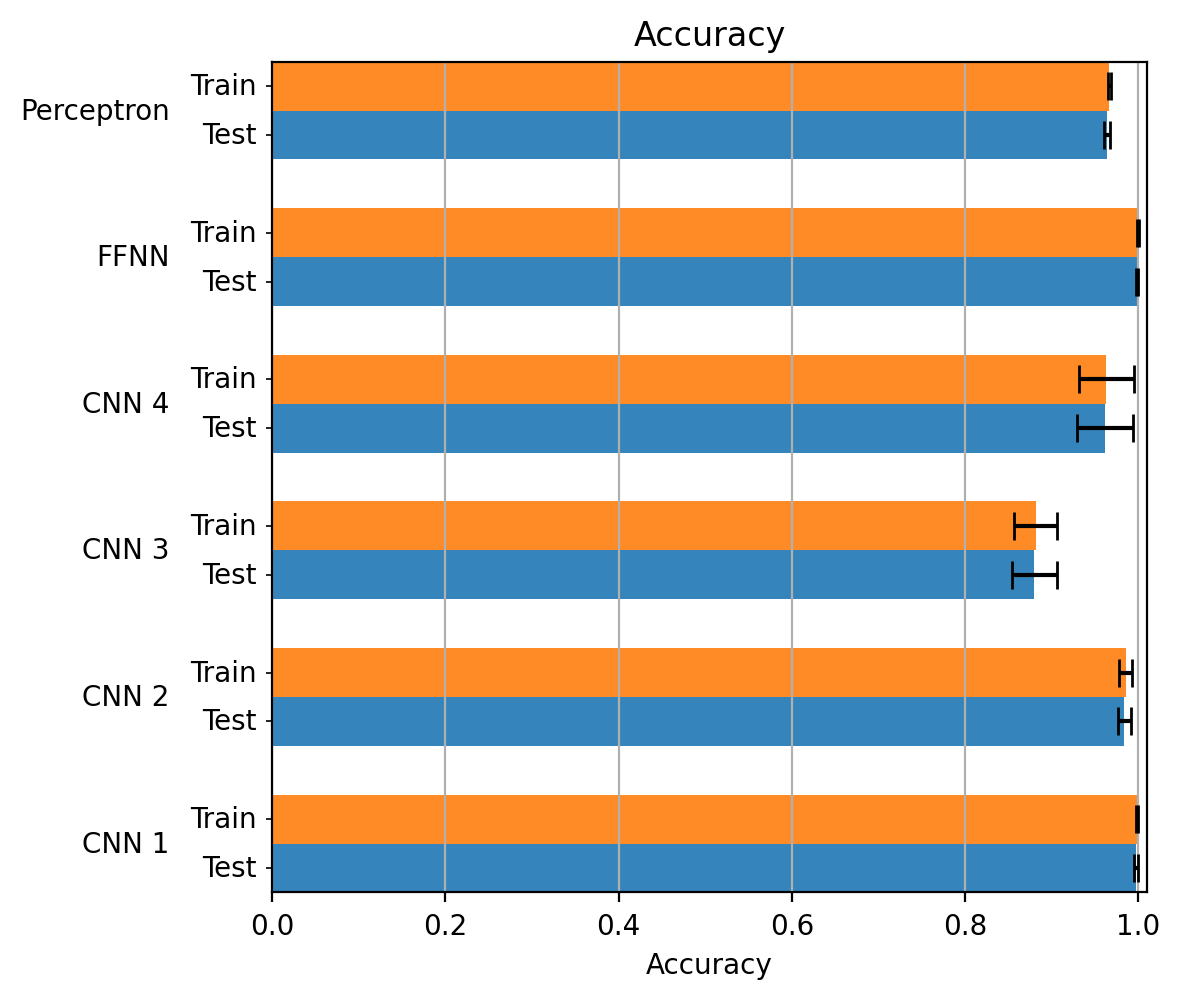
\includegraphics[width=0.85\linewidth]{../images/accuracy.png}
	\caption{Accuracy and its standard deviation results for training and test sets}
\end{figure}

\textbf{Loss function value}
\begin{longtable}[]{@{}lll@{}}
	\toprule
	\textbf{Models} & \textbf{Training} & \textbf{Test}\tabularnewline
	\midrule
	\endhead
	Perceptron & mean = 0.1529 & mean = 0.1584\tabularnewline
	& STD = 0.0043 & STD = 0.0069\tabularnewline
	FFNN & mean = 0.0095 & mean = 0.0109\tabularnewline
	& STD = 0.0051 & STD = 0.0053\tabularnewline
	CNN\_1 & mean = 0.0139 & mean = 0.0169\tabularnewline
	& STD = 0.005 & STD = 0.0071\tabularnewline
	CNN\_2 & mean = 0.0511 & mean = 0.0551\tabularnewline
	& STD = 0.0214 & STD = 0.0206\tabularnewline
	CNN\_3 & mean = 0.3454 & mean = 0.3487\tabularnewline
	& STD = 0.0659 & STD = 0.0664\tabularnewline
	CNN\_4 & mean = 0.1103 & mean = 0.117\tabularnewline
	& STD = 0.0885 & STD = 0.09\tabularnewline
	\bottomrule
	\caption{Loss function and its standard deviation results for training and test sets}
\end{longtable}



\begin{figure}[h!]
\centering
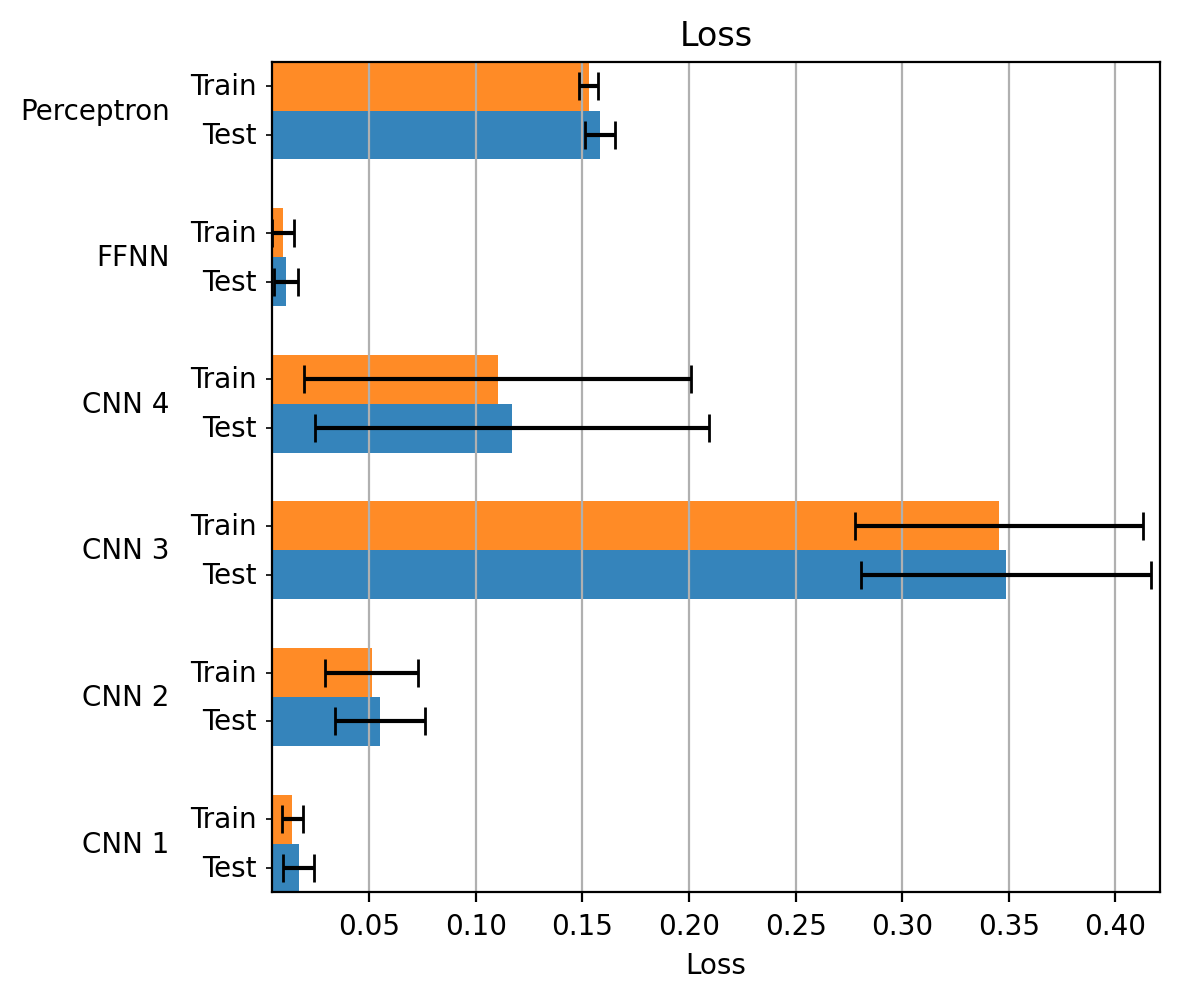
\includegraphics[width=0.85\linewidth]{../images/loss.png}
\caption{Loss function and its standard deviation results for training and test sets}
\end{figure}

\subsection{Metrics during training phase}\label{header-n613}

The following graphs show the trend of the metric for each model during
the training phase, calculated both on the training and test sets.

\textbf{Perceptron}

\begin{figure}[h!]
\centering
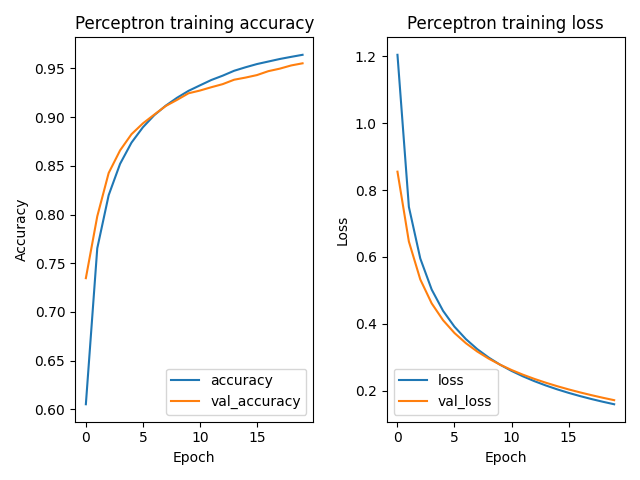
\includegraphics[width=0.68\linewidth]{../images/perceptron_training_accuracy.png}
\caption{\emph{Perceptron} accuracy and loss function value during training phase}
\end{figure}

\textbf{FFNN}

\begin{figure}[h!]
\centering
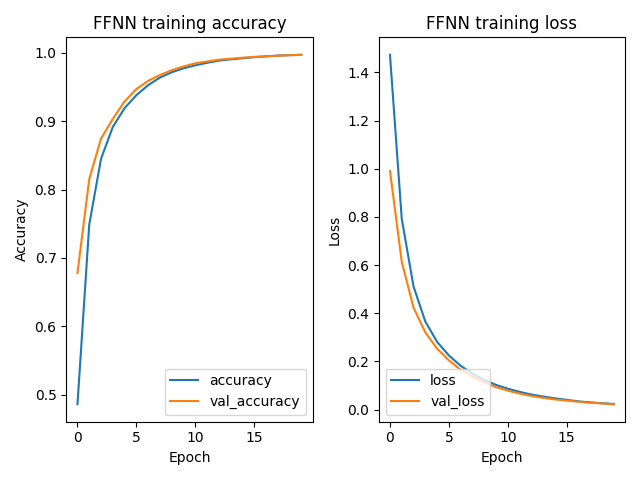
\includegraphics[width=0.68\linewidth]{../images/ffnn_training_accuracy.png}
\caption{\emph{FFNN} accuracy and loss function value during training phase}
\end{figure}

\textbf{CNN\_1}

\begin{figure}[h!]
\centering
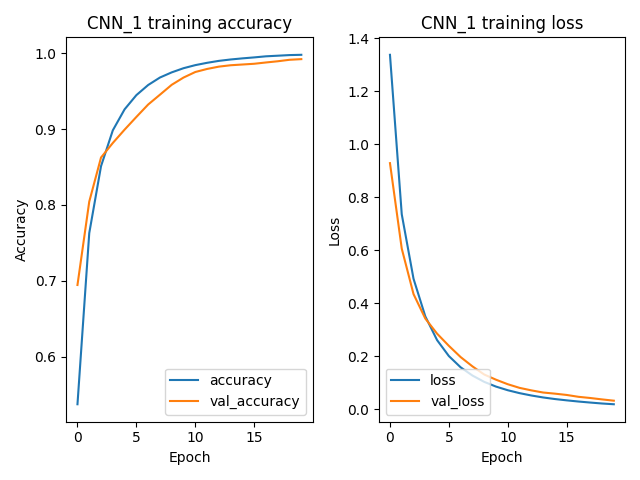
\includegraphics[width=0.68\linewidth]{../images/cnn_1_training_accuracy.png}
\caption{\emph{CNN\_1} accuracy and loss function value during training phase}
\end{figure}

\textbf{CNN\_2}

\begin{figure}[h!]
\centering
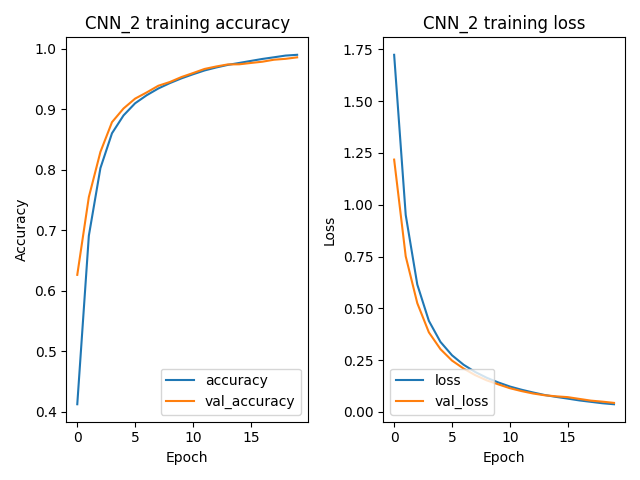
\includegraphics[width=0.68\linewidth]{../images/cnn_2_training_accuracy.png}
\caption{\emph{CNN\_2} accuracy and loss function value during training phase}
\end{figure}

\newpage

\textbf{CNN\_3}

\begin{figure}[h!]
\centering
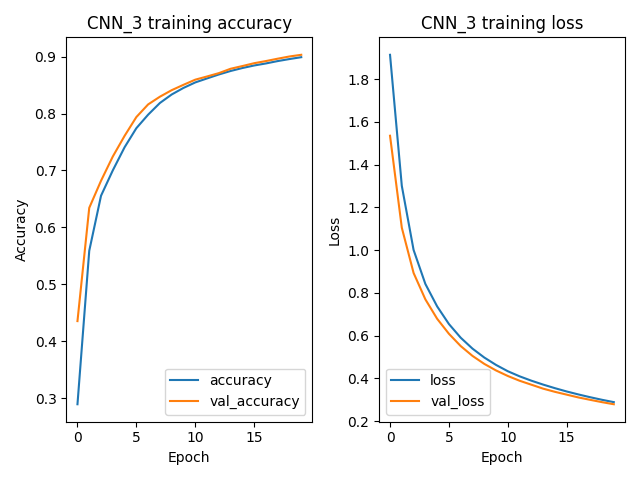
\includegraphics[width=0.68\linewidth]{../images/cnn_3_training_accuracy.png}
\caption{\emph{CNN\_3} accuracy and loss function value during training phase}
\end{figure}

\textbf{CNN\_4}

\begin{figure}[h!]
\centering
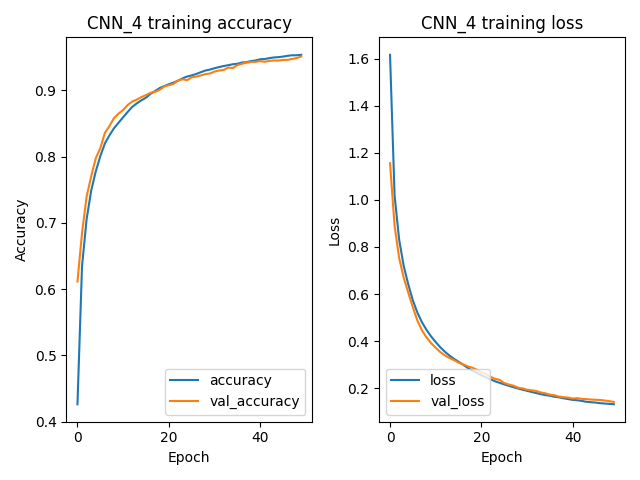
\includegraphics[width=0.68\linewidth]{../images/cnn_4_training_accuracy.png}
\caption{\emph{CNN\_4} accuracy and loss function value during training phase}
\end{figure}

\subsection{Observations}\label{header-n627}

The following observations are statistically validated using the
Wilcoxon test.

\emph{1) All neural networks used to execute the experiments performs
well.} The models get high accuracy results and low loss function
values. Their performances are great even if the training phase short:
the number of epochs is 20 for all models, with the exception of
\emph{CNN\_4} for which the number of epochs is 50. In particular, the
accuracy is always greater than 0.85, and the loss values smaller than
0.35.

\emph{2) Task simplicity requires simple models.} In general, the
models' performances degrade with an increase in complexity. The
simplest model (the \emph{Perceptron}) works better than the most
complicated one (\emph{CNN\_3}). The complexity of the latter requires a
longer training phase to increase its performance. The prove of this is
\emph{CNN\_4}, which has the same architecture as \emph{CNN\_3}, but the
number of epochs is higher and the batch size lower. In this way, the
model can learn more and faster. Despite this, the standard deviation
grows both for accuracy and loss function value: the network performance
strongly depends on the holdout used for training the network.

\emph{3) The overfitting problem does not exist.} No model produces
overfitting, even the most complex ones. This means that data is simply
to learn and all of them are characterize from common patterns.

\emph{4) FFNN is the best model.} The Wilcoxon test confirms that
\emph{FFNN} is the network with higher performance in the validation
phase, overcoming also \emph{CNN\_1}. Despite this is true both for
accuracy and loss function value, it is more visible in the loss
function graphic.

\emph{5) CNN\_3 is the worst model.} This network has lower performance,
both for the training and validation phase, because the reduced number
of epochs does not allow the complex architecture of the network to
learn enough.

\section{Conclusions}\label{header-n631}

The image multi-classification task described in this project is
relatively simple if it is addressed using deep learning models. The two
main reasons concern the dataset characteristics and the task's
simplicity. The dataset is composed of pictures that depict only the
fruit and vegetables to classify, without other objects that can add
noise. In this way, the models learn only the feature that characterizes
the target classes. In addition, the images represent the subject in
different positions and light conditions. This fact allows to avoid the
image augmentation technique during the pre-processing phase. Simple
models work better because of the task's simplicity. Compared to more
complex models, their performance is higher, they learn faster and the
standard deviation is lower. The best one is a simple feed-forward
neural network, which works better than all convolutional neural network
tested in the experiments.

\end{document}



\end{document}